\documentclass[12pt]{article}
\usepackage{amsmath}
\usepackage{jheppub}
\usepackage{marginnote,xparse,changepage,caption}

\newcommand{\IGNORE}[1]{}
\newcommand{\be}{\begin{equation}}
\newcommand{\ee}{\end{equation}}
\newcommand{\bea}{\begin{aligned}}
\newcommand{\eea}{\end{aligned}}
\newcommand{\mb}[1]{\marginnote{\texttt{\small MB:\,#1}}}
\renewcommand{\ij}[1]{\marginnote{\texttt{\small IJ:\,#1}}}
\newcommand{\ibar}{{\overline{\emph\i}}}
\newcommand{\jbar}{{\overline{\emph\j}}}
\newcommand{\mnote}[1]{\marginpar{\raggedright \scriptsize   #1 } }

\title{Boundary terms in the action for Causal Sets}
 \author[a]{Michel Buck}
 \author[a,b]{\!, Fay Dowker}
 \author[a]{ Ian Jubb\,}
 \author[c]{and Sumati Surya}
\affiliation[a]{Theoretical Physics Group, Blackett Laboratory, Imperial College, London, SW7 2AZ, U.K.}
\affiliation[b]{Institute for Quantum Computing, University of Waterloo, ON, N2L 2Y5, Canada}
\affiliation[c]{Raman Research Institute, CV Raman Ave, Sadashivanagar, Bangalore 560080, India}
\abstract{ 
We propose a family of formulae for the boundary term in the action of a causal set that is well-approximated by a continuum manifold with spacelike boundary. %The boundary term is proportional to the difference in the number of elements immediately to future and the number of elements immediately to the past of the surface. 
We show that in the continuum limit one recovers the Gibbons-Hawking-York boundary term in the mean.
}

\begin{document}

\maketitle

\section{Introduction}

%[MB1: USEFUL QUOTE FROM RAFAEL: In the quantum theory, however, these boundary terms are important. They are essential in order that the quantum mechanical amplitudes satisfy the correct composition law and in order that these amplitudes have the correct classical limit. In a number of examples [5] they give a contribution to the partition function which is important for the agreement with calculations based on straightforward thermodynamics. In this note we shall derive the boundary terms in the action for the Regge calculus]

In furthering causal set theory it is crucial that we understand the kinematics of the theory. The action of a given causal set is a crucial piece of the kinematics that would be extremely useful to know and understand. Proposals for the action of a causal set are available \cite{Benincasa_Dowker:The_Scalar_Curvature_of_a_Causal_Set} and these hold analytically in some cases and numerically in many more.\mb{rephrase} These cases being when the causal set is embeddable in some existing spacetime. One can show that the action of the causal set then agrees with the Einstein-Hilbert action of the spacetime in some continuum limit. How this limiting procedure is carried out will be described in more detail below.

It is well known that the Einstein-Hilbert action is not the full story in the continuum. In the presence of spacetime boundaries the gravitational action must include a boundary term $S_{GHY}$, the Gibbons-Hawking-York action, in order to yield a well-defined variational principle~\cite{Gibbons_Hawking_Boundary}. The contributions of this term play an essential role in particular in the quantum theory. For instance, in the calculation of the black hole entropy via the Euclidean path-integral, it is the boundary terms that produce the answer $A/4l_p^2$ necessary for the unification of black hole mechanics with thermodynamics. To give another example, in Regge calculus boundary terms are necessary in order that the quantum mechanical amplitudes satisfy the correct composition law and that they have the correct classical limit~\cite{hartlesorkin}.\mb{is this true?}

We define a \textit{causal set} (or \textit{causet}) as a locally finite partial order. This means it is a pair $(\mathcal{C},\preceq)$ where $\mathcal{C}$ is the set of points and $\preceq$ is a partial order relation on $\mathcal{C}$ that has the following properties. It is (i) reflexive: $x\preceq x$, (ii) acyclic: $x\preceq y\preceq x \Rightarrow x=y$, and (iii) transitive: $x\preceq y\preceq z \Rightarrow x\preceq z$ for all points $x, y, z \in \mathcal{C}$. We define an inclusive order interval as the set $I(x,y)\equiv \lbrace z\in\mathcal{C}|x\preceq z\preceq y\rbrace$ for any $x, y\in\mathcal{C}$. The \textit{locally finite} condition is simply that the cardinality of any order interval is finite, that is $|I(x,y)|<\infty$. This condition ensures we are dealing with a discrete structure, as all the other properties of the relation would apply to an order relation between points on a continuous manifold.

In order to say we have a causal set analogue for a continuous expression we need a well defined procedure for relating the discrete theory to the continuum. This procedure, or tool, is called a \textit{Poisson sprinkling}, or just a \textit{sprinkling}. It is a Poisson process which provides a way to generate a causet from a $d$-dimensional Lorentzian manifold $(\mathcal{M},g)$ by selecting points in $\mathcal{M}$ to be the elements of $\mathcal{C}$, with an order relation given by the causal order of the manifold. The number of points chosen in a region of spacetime volume, $V$, is a Poisson random variable. This means that the expected number of points in some region will be $\rho V$, where $\rho$ is the density of the sprinkling. The density is related to the discreteness scale, $l$, by $\rho=l^{-d}$ in $d$ spacetime dimensions. It is called a sprinkling as one can envisage the point selection process as a `sprinkling' of points into the manifold. If a causet, $\mathcal{C}$, can be generated with relatively high probability by a sprinkling into the manifold, $(\mathcal{M},g)$, then we say that the manifold is a good approximation for the causal set.

\section{The Claims}

Consider a sufficiently well-behaved $d$-dimensional spacetime $(M,g)$ and Cauchy surface $\Sigma$ in $M$. The causal past and future sets $M^\pm=J^\pm(\Sigma)$ form a partition of $M$ and $\partial M^\pm = \Sigma$. The Gibbons-Hawking-York boundary term for $M^\pm$ is in this case given by
\be\label{eq:GHYBT_in_continuum}
S_{GHY} = \pm \frac{1}{l_p^{d-2}}\int_{\Sigma} K d\Sigma
\ee
where $l_p$ is the rationalised Planck length and $K$ is the trace of the extrinsic curvature $K_{\mu\nu}=h_{\mu}^\rho h_\nu^\sigma \nabla_\rho n_\sigma$ of $\Sigma$ defined with future-pointing timelike unit normal $n_{\mu}=\partial_\mu S/\sqrt{g^{\mu\nu}\partial_\mu S\partial_\nu S}$. (We will work with a mostly plus convention for the metric, in which this translates into a past-pointing normal vector $n^{\mu}$).\mb{ok or more detail on conventions needed?}

Now observe that the integral in~\eqref{eq:GHYBT_in_continuum} can be thought of as the ``volume gradient'' across the surface $\Sigma$. More formally
\be
\int K d\Sigma = \frac{\partial}{\partial n}\int d\Sigma,
\ee
where the right hand side is the derivative of the area $\int d\Sigma$ as each point of $\Sigma$ is moved an equal distance along the unit normal vector, $n^{\mu}$, which corresponds to the rate of change of the surface volume backwards in time, as $n^{\mu}$ is past-pointing. 
\mb{does the antichain analogy really stand?} 
In the causal set, the analogue of a spacelike hypersurface is an anti-chain, i.e. a subset $\mathcal{A}\subseteq\mathcal{C}$ in which all elements are unrelated. The intuitive analogue of the boundary term would then be the rate of change of the number of causal set elements below and above the antichain. We shall see that this intuitive idea indeed bears out. %This suggests a very simple analogy for a causal set with a ``spacelike hypersurface''. \mb{under construction} The analogy These unrelated elements are maximal in the sense that there exist no elements $y\in\mathcal{C}\setminus\mathcal{A}$ such that $x\preceq y$, $\forall x\in\mathcal{A}$. 

Consider a causal set $\mathcal C$ obtained by a Poisson sprinkling at density $\rho=1/l^d$ into a $d$-dimensional spacetime $(M,g)$. A Cauchy surface $\Sigma\subset M$ induces a partition $\mathcal C = \mathcal C^+ \cup\, \mathcal C^-$ of the sprinkling, where $\mathcal C^+$ and $\mathcal C^-$ denote the restrictions of $\mathcal C$ to the points sprinkled to the future and past of $\Sigma$, respectively. Spacetime volume in the causal set is obtained simply by counting the number of elements, and hence the volume gradient corresponds to the difference in the number of ``immediate neighbours'' to the future and to the past of the surface. The most natural definition for the nearest neighbours to the future/past of $\Sigma$ in the sprinkling is to take the minimal/maximal elements in $\mathcal C^\pm$, respectively. Thus $x\in \mathcal C^-$ is a maximal element in $\mathcal C^-$ if it is maximal in the precedence relation of the causal set, i.e. if there exists no element $y\in\mathcal C^-$ such that $x\preceq y$. Figure \ref{fig:Nmin_Nmax} shows an illustration of the idea. The minimal and maximal elements have been highlighted. 
%in COLOUR.

We will also show that it is possible to restrict oneself to either $\mathcal C^+$ or $\mathcal C^-$ and still calculate the GHY term. To do this requires us to define the $k$-next-to-maximal/minimal elements in $\mathcal C^-$ or $\mathcal C^+$ respectively. These are the elements of the causal set that have $k$ elements to their future or past. This means that the $0$-to-maximal/minimal elements are the maximal/minimal elements. 
%Elements with $1$ element to their past/future have been highlighted in COLOUR in Figure \ref{fig:Nmin_Nmax}, and those with $2$ have been highlighted in COLOUR.

Let us denote the number of $k$-next-to-maximal elements in $\mathcal C^-$ by $N_{max}^{(k)}$ and the number of $k$-next-to-minimal elements in $\mathcal C^+$  by $N_{min}^{(k)}$. We propose the following definitions for the discrete Gibbons-Hawking-York boundary term (one can adopt the appropriate definition to best suit their calculation needs):\mb{put $\Sigma$ in argument, $S[\mathcal C, \Sigma]$?}

\be\label{GH_boundary_to_causet}
 \mathcal{S}^{(d)}_{GHY}[\mathcal C]=\left(l/l_p\right)^{d-2}\frac{c_{d}}{\Gamma\left(\frac{2}{d} \right)}\times
  \begin{cases}
   \frac{1}{2}\left(N_{max}^{(0)}-N_{min}^{(0)}\right) \\
   d\: N_{max}^{(1)}-N_{max}^{(0)} \\
   N_{min}^{(0)}-d\: N_{min}^{(1)}
  \end{cases}
\ee
where the constant $c_{d}$ only depends on the spacetime dimension and is given by
\be\label{Cn}
c_{d}=\frac{d(d+1)}{(d+2)}\left[\frac{A_{d-2}}{d(d-1)}\right]^{\frac{2}{d}},
\ee
$A_d=2\pi^\frac{d+1}2/\Gamma\left(\frac{d+1}{2}\right)$ and denotes the volume of the unit $d$-sphere. In fact, one can write down a general expression for the boundary term as a sum over $k$  $N_{\vphantom{i}max}^{\: (k)}$ and/or $N_{min}^{\: (k)}$ terms with particular coefficients. This can be written as follows:

\begin{gather}\label{general_boundary_sum}
\begin{aligned}
\mathcal{S}^{(d)}_{GHY}[\mathcal C]=\left(l/l_p\right)^{d-2} & c_{d}\left( \sum_m p_m \frac{\Gamma\left(\frac{2}{d}+m \right)}{\Gamma\left(\frac{1}{d}+m \right)}  - \sum_n q_n\frac{\Gamma\left(\frac{2}{d}+n \right)}{\Gamma\left(\frac{1}{d}+n \right)} \right)^{-1} \\
& \times \left( \sum_m p_m \frac{m!}{\Gamma\left(\frac{1}{d}+m \right)} N_{max}^{(m)}
+  \sum_n q_n \frac{n!}{\Gamma\left(\frac{1}{d}+n \right)} N_{min}^{(n)}\right)
\end{aligned}
\end{gather}
The coefficients, $p_m , q_n \in \mathbb{R}$, must satisfy the following relation:

\be\label{coefficient_relation}
\sum_m p_m + \sum_n q_n = 0
\ee
The different definitions of the boundary term in (\ref{GH_boundary_to_causet}) are just simple cases of this general formula, and the objects that one would preferably use in a calculation. From above one can see that at least two terms are needed in the sum to find the boundary term. The condition~\eqref{coefficient_relation} means that there will be one free parameter if two terms are present\footnote{For example you could include only the maximal and minimal terms (like the first case in~\eqref{GH_boundary_to_causet}) with $p_0=p$ and $q_0=-p$ where $p\in\mathbb{R}$. This would satisfy~\eqref{coefficient_relation} and would leave $p$ as a free parameter. In this case you would get a factor of $p^{-1}$ from the term after $c_d$ in~\eqref{general_boundary_sum} which will cancel the $p$ from the last term.}. This free parameter will be cancelled by the term after $c_d$ in~\eqref{general_boundary_sum}. Thus, with only two terms, the form of the discrete boundary term is fixed. If one chooses to include more than two terms the coefficients of the $N_{{max\vphantom{i}}}^{\:(k)}$ and/or $N_{{min}}^{\:(k)}$ terms are no longer unique.

To support this proposal we show that in the continuum limit of $l\rightarrow 0$ (i.e. $\rho\rightarrow\infty$) we obtain
%of infinite sprinkling density into a $d$-dimensional spacetime we obtain
\be
\lim_{l\rightarrow0}\langle S^{(d)}_{GHY}[\mathcal C] \rangle= \frac{1}{l_p^{d-2}}\int_{\Sigma} d^{d-1}x\: \sqrt{h}\: K\label{eq:mainconjecture}
\ee
for the most general definition above. Here $\langle\cdot\rangle$ denotes the mean over sprinklings.

We also propose a discrete definition for the spatial volume of the surface:

\be\label{eq:surface_volume}
\mathcal{A}^{(d)}[\mathcal{C}]=\left(l/l_p\right)^{d-1}\frac{b_{d}}{\Gamma\left(\frac{1}{d}\right)}\: N_{{\,}_{max/min}}^{\:(0)}
\ee
where the constant $b_d$ is given by

\be\label{constant_b_d}
b_d=d\left[\frac{A_{d-2}}{d(d-1)}\right]^{\frac{1}{d}}
\ee
Again on can find a general expression written as a sum of different terms.

\be\label{general_area_sum}
\mathcal{A}^{(d)}[\mathcal{C}]=\left(l/l_p\right)^{d-1}b_{d}\sum_m p_m \frac{m!}{\Gamma\left(\frac{1}{d}+m \right)}\: N_{{\,}_{max/min}}^{\:(m)}
\ee
where the coefficients, $p_m$, must satisfy $\sum_m p_m =1$. This time we see that only one term is needed to find the surface volume, and that when more than one term is added the coefficients will not be unique. We support this claim in the same way as the boundary term, and show that

\be\label{eq:conjecture_for_area}
\lim_{l\rightarrow0}\langle \mathcal{A}^{(d)}[\mathcal{C}] \rangle= \frac{1}{l_p^{d-1}}\int_{\Sigma} d^{d-1}x\: \sqrt{h}
\ee
where the right hand side is the spatial volume of the surface $\Sigma$.

%MB1: (too vague) During the calculation approximations will be made. These approximations are justified on the grounds that if certain orders are retained throughout the calculation they will in fact vanish in the limit $\rho \rightarrow \infty$
\begin{figure}
  \centering
    {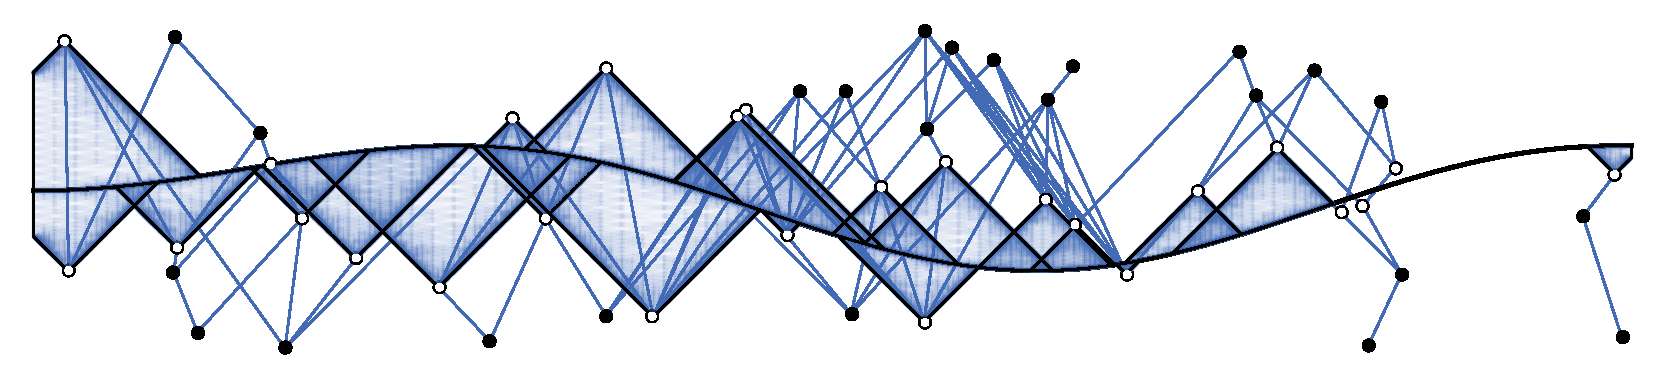
\includegraphics[width=\textwidth]{minmaxplot}}
     \caption{An illustration of the idea. Pictured here is a causal set obtained by a sprinkling into a spacetime partitioned by a spacelike hypersurface. The minimal and maximal points about the surface are highlighted and the shaded regions illustrate the regions whose volumes $V_\blacktriangle$ and $V_\blacktriangledown$ are needed in the proof.}
     \label{fig:Nmin_Nmax}
\end{figure}

\section{The Proof}

\subsection{Poisson Sprinklings for $\langle N_{max}^{(m)}\rangle$ and $\langle N_{min}^{(m)}\rangle$}

In order to prove~\eqref{eq:mainconjecture} and~\eqref{eq:conjecture_for_area} let us first derive expressions for the mean values of $N_{max}^{(m)}$ and $N_{min}^{(m)}$. For any instance of the sprinkling, the probability that a sprinkled point $p\in M$ below the surface $\Sigma$ is $k$\emph{-next-to-maximal} is given by the probability that $k$ points of the sprinkling lie in the region $J^{+}(p)\cap J^{-}(\Sigma)$, the intersection of the causal future of $p$ with the causal past of the surface $\Sigma$.\footnote{For notational convenience we use the symbol $x$ to refer to the causal element $x\in\mathcal C$, to its embedding in the manifold $M$, and to its coordinates in some chart on $M$.} This region will in general be the interior of some curvy $d$-dimensional cone truncated by the surface $\Sigma$, as illustrated in Figure~\ref{fig:Nmin_Nmax}. We will refer to these regions as \emph{truncated cones} below. The Poisson process assigns a probability
\be\label{Poisson}
\mathbb P\left(\text{k points in }J^{+}(p)\cap J^{-}(\Sigma)\right)=\frac{\left(\rho\: V_\blacktriangledown(p)\right)^k}{k!}e^{-\rho V_\blacktriangledown(p)}
\ee
to this event, where $V_\blacktriangledown(p)\equiv V(J^{+}(p)\cap J^{-}(\Sigma))$ is the spacetime volume of the region $J^{+}(p)\cap J^{-}(\Sigma)$. The probability of sprinkling an element into an infinitesimal four-volume $dV_p$ at $p$ is $\rho dV_p$ where $\rho=l^{-d}$ is the sprinkling density, and so the total expected number of $k$-next-to-maximal elements below $\Sigma$ is
\be\label{eq:nmax}
\langle N_{max}^{(k)}\rangle =\rho\int_{J^{-}(\Sigma)}dV_p\; \frac{\left(\rho\: V_\blacktriangledown(p)\right)^k}{k!}e^{-\rho V_\blacktriangledown(p)}
\ee
Similarly the expected number of $k$-next-to-minimal elements above $\Sigma$ is
\be\label{eq:nmin}
\langle N_{min}^{(k)}\rangle =\rho\int_{J^{+}(\Sigma)}dV_p\; \frac{\left(\rho\: V_\blacktriangle(p)\right)^k}{k!}e^{-\rho V_\blacktriangle(p)}
\ee
where $V_\blacktriangle(p)\equiv V(J^{+}(\Sigma)\cap J^{-}(p))$.

In the limit $\rho\rightarrow\infty$, both quantities will diverge, but if some combination of maximal and minimal terms grows slower than or at order $\rho^{1-\frac2d}$, the proposed action~\eqref{general_boundary_sum} will tend to a finite value in the continuum limit.

Consider a set of synchronous or Gaussian Normal Coordinates (GNC) $x^\mu=(t,\mathbf x)$ adapted to $\Sigma$ such that in a neighbourhood $U_\Sigma$ of $\Sigma$ the line element is
\be
ds^2 = -dt^2 + h_{ij}(t,\mathbf x) dx^i dx^j.
\ee
In these coordinates, the surface $\Sigma$ corresponds to $t=0$, and the coordinate $t$ measures the proper time elapsed along geodesics whose tangent vector is proportional to the surface normal on $\Sigma$.
%\be\label{GNC_metric}
%g_{\mu\nu}(x)=
%\begin{pmatrix}
 %-1&0 \\
% 0&h_{ij}(x)
%\end{pmatrix}.
%\ee
%In order to find $N_{max}$, the number of maximal points below the surface, one has to use the fact that the points have been sprinkled with a Poisson distribution. 
%If we pick a point $x_0=(0,\mathbf{x})\in \Sigma$ on the surface that has the same spatial coordinates as $x=(t,\mathbf{x})$ then the coordinate time, $t$, is the proper time elapsed along the unique geodesic between $x_0$ and $x$. The volume $V(\Sigma,x)$ then only depends on $t$.~\mb{error?}  
The integrals~\eqref{eq:nmax} and ~\eqref{eq:nmin} seem intractable as they stand, since the integration is over the entire causal past/future of the surface and the volume expressions will be complicated in the presence of curvature. However, for large $\rho$ (small $l$), the integrands $\exp(-\rho V)$ will be exponentially suppressed unless the volumes are small. Consider the spacetime region $U_\varepsilon=\left\{|t|<\varepsilon\right\}$ around the surface $\Sigma$ for some $\varepsilon>0$ (with $\varepsilon$ small enough such that the GNC system is valid throughout $U_\varepsilon$). We will assume that for any such $\varepsilon$, the contribution from points with $|t|>\varepsilon$ to the integrals~\eqref{eq:nmax} and \eqref{eq:nmin} can be made arbitrarily small by setting $\rho$ large enough, since the volumes of the truncated past/future lightcones for such points will be too large. Hence, as $\rho\rightarrow\infty$, the integration ranges in \eqref{eq:nmax} and \eqref{eq:nmin} can be cut off at finite time $t=\pm\varepsilon$ with $\varepsilon$ arbitrarily small, which allows us to expand the time integration-variable about zero. These assumptions of course impose certain regularity conditions on the surface $\Sigma$, but we will assume that they are reasonable conditions.\mb{do we need to say more about this? e.g. can't have asymp. null $\Sigma$ i guess} The integrals then simplify to
\begin{gather}\label{eq:nmax_and_eq:nmin}
\begin{aligned}
\langle N_{max}^{(k)}\rangle & =\rho \int_{\Sigma}d^{d-1}x\int_{-\varepsilon}^{0}dt\:
h^{\frac{1}{2}}\left(1+
\frac{1}{2}\frac{\dot{h}}{h}t+O(t^2)\right)
 \frac{\left(\rho\: V_\blacktriangledown(p)\right)^k}{k!} e^{-\rho V_\blacktriangledown(t,\mathbf x)}
\\
\langle N_{min}^{(k)}\rangle & =\rho \int_{\Sigma}d^{d-1}x\int_{0}^{\varepsilon}dt\:
h^{\frac{1}{2}}\left(1+
\frac{1}{2}\frac{\dot{h}}{h}t+O(t^2)\right) \frac{\left(\rho\: V_\blacktriangle(p)\right)^k}{k!} e^{-\rho V_\blacktriangle(t,\mathbf x)}
\end{aligned}
\end{gather}
where $h\equiv det\left(h_{ij}(0,\mathbf{x})\right)$ and $\dot{}\equiv \frac{\partial}{\partial t}$ and the metric determinant has been in expanded in small $t$.

The only truncated cones that contribute will have small volumes, as we are restricting ourselves close to the surface.
%\mb{this sounds circular w.r.t. last paragraph} 
This means that the volumes can be approximated by the volumes of less curvy cones, and it can be shown that higher order corrections, in the approximation scheme, vanish in the limit of $\rho \rightarrow \infty$. This will all be made more precise below.

\subsection{Lightcone Volumes}

In order to evaluate the volume $V_\blacktriangledown(p)$ or $V_\blacktriangle(p)$ of a truncated cone we will perform a coordinate transform to Riemann Normal Coordinates (RNCs) in a neighbourhood containing the cone. The discussion for the two volume integrals is identical so we will outline that for $V_\blacktriangle(p)$ (i.e. for points to the future of $\Sigma$). 

Fix $p\in M$ and denote its coordinate values in GNCs by $x^\mu_p=(t_p,\mathbf x_p)$. It will be convenient to use RNCs centered not at the tip $p$ of the cone but instead at the point $p_0$ where the unique geodesic through $p$ whose tangent is normal to $\Sigma$ intersects $\Sigma$. In GNCs this simply corresponds to the point $p_0$ with coordinates $x_0^\mu=x^\mu(p_0)=(0,\mathbf x_p)$. RNCs centered at $p_0$ will be given the symbol $y^{\overline{\mu}}$.
%\mb{let's put all facts about $x^\mu$ and $y^{\overline\mu}$ for $p$ and $p_0$ here and expansion of det in RNC.} 
We need to assume that for any $p$ in $U_\varepsilon$, the Riemann normal neighbourhood $U_p\subset M$ (throughout which the RNC system centered at $p_0$ is well-defined) contains the truncated cone $J^-(p)\cap J^+(\Sigma)$. This assumption seems reasonable given the that $U_\varepsilon$ can be made arbitrarily ``thin'' as $\rho\rightarrow\infty$. In RNCs the metric and the Christoffel symbols at $p_0$ are those of flat space:
\be\label{eq:RNCMetricTransAtPAndChris}
g_{\overline{\mu} \overline{\nu}}(p_0)=\eta_{\overline{\mu} \overline{\nu}}=A^{\mu}_{\;\overline{\mu}}A^{\nu}_{\;\overline{\nu}}g_{\mu\nu}(p_0)\;,\;\;\;\;\Gamma^{\overline{\mu}}_{\;\overline{\nu}\overline{\rho}}(p_0)=0
\ee
The $A^{\mu}_{\;\overline{\mu}}$ govern the coordinate transformation from GNCs to RNCs to linear order. %but $O(x^2)$ corrections may be required. 
To second order the coordinate transformation is given by
\be\label{eq:RNCtotaltrans}
y^{\overline{\mu}}=A^{\overline{\mu}}_{\;\nu}x^\nu+\frac{1}{2}A^{\overline{\mu}}_{\;\mu}\Gamma^{\mu}_{\;\nu\rho}(p_0)x^\nu x^\rho+O((x-x_0)^3).
\ee
The inverse relation to first order is 
\be\label{eq:RNCinversetrans}
x^{\mu}=A^{\mu}_{\;\overline{\nu}}y^{\overline{\nu}}+O(y^2)
\ee
and one finds that the $A^{\mu}_{\;\overline{\mu}}$ satisfy
\be\label{eq:RNCeqnforA}
A^{\overline{\mu}}_{\;\mu}A^{\mu}_{\;\overline{\nu}}=\delta^{\overline{\mu}}_{\;\overline{\nu}}\;,\;\;\;\;A^{\mu}_{\;\overline{\mu}}A^{\overline{\mu}}_{\;\nu}=\delta^{\mu}_{\;\nu}
\ee
These relations for RNC will cover all that will be needed in this discussion.

Now the volume of the truncated cone can be found as follows. 
%Consider the past lightcone emanating at the point $p_0=(T,\mathbf x_0)$ truncated by $\Sigma$. There is a unique point $q_0=(0,\mathbf x_0)$ on $\Sigma$ associated with $p_0$, separated from $p_0$ by proper time $T$. 
The volume of the cone is given by

\be\label{eq:VolumeWithNoSimplifications}
V_\blacktriangle(p)=\int_{\mathcal{X}_p} d^d x\;\sqrt{-g}
\ee
where the integration region, $\mathcal{X}_p\equiv  J^-(p)\cap J^+(\Sigma)$ will be a complicated expression. As we are dealing with points close to the surface we can use the  RNCs $y^{\overline{\mu}}$, defined as above, about the point $p_0$. Let us denote the time-coordinate of $p$ in GNCs by $T=x^0_p=t_p$. For the transformation from GNCs to RNCs at $p_0$ one finds that $A^{\overline 0}_{\;0}=1$, $A^{\overline 0}_{\;i}=0$ and $\delta_{\ibar\jbar}=A^i_{\;\ibar}A^j_{\;\jbar}h_{ij}(p_0)$, which in particular implies $y^{\overline{0}}_p=\overline{t}_p=t_p=T$. In RNC one can expand the metric determinant in~\eqref{eq:VolumeWithNoSimplifications} to find

\be\label{eq:VolumeWithRNC}
V_\blacktriangle(p) =\int_{\mathcal{X}_p}d^dy+\int_{\mathcal{X}_p}d^dy\left(-\frac{1}{6}R_{\overline{\mu}\overline{\nu}}(p_0)y^{\overline{\mu}}y^{\overline{\nu}} \right)+O(T^{d+3})
\ee
where $R_{\overline{\mu}\overline{\nu}}(p_0)$ is the Ricci tensor in RNC evaluated at $p_0$.\mb{justify beforehand which orders to keep?}
%The arguments of the volume function need not be changed as the volume only depends on the points in the manifold, $q_0$ and $p_0$. 
The second term comes in at $O(T^{d+2})$ so the volume we have to calculate has reduced to

\be\label{eq:VolumeToLowestOrder}
V_\blacktriangle(p) =\int_{\mathcal{X}_p}d^dy+O(T^{d+2})
\ee
Terms of $O(T^{d+2})$ can be retained till the end, but in the limit, $\rho\rightarrow\infty$, they vanish. This will be proved below.

This is now a simple volume integral but we need to find the boundaries of $\mathcal{X}_p$ to write down the integration limits. There are two boundaries to the (solid) truncated cone: the lightcone emanating at $p$ and the base, given by the intersection of $\Sigma$ with the interior of the lightcone. First we look at the lightcone. Following \cite{Khetrapal_Sumati:Causal_Diamond_Volume} it can be shown that the first curvature correction to the lightcone comes in at $O(T^{d+2})$ and so can be ignored for our purposes. This means that the lightcone can be treated as effectively flat in RNCs and thus corresponding to the set $(y^{\overline{1}})^2+(y^{\overline{2}})^2+...+(y^{\overline{d-1}})^2= T-\overline{t}$.\mb{what limit on $\bar t$?}

The base of the cone in GNCs is simply a part of the surface $t=0$, so we can use (\ref{eq:RNCtotaltrans}) to find the equation for the surface in RNCs. Equation (\ref{eq:RNCtotaltrans}) gives

\be\label{eq:BottomSurfaceWithGNC}
\overline{t}=\frac{1}{2}\Gamma^{0}_{\;ij}(p_0)x^i x^j+O( x^3)\ee

The linear part on the right of (\ref{eq:RNCtotaltrans}) vanishes as $A^{\overline{0}}_{\;\mu}x^{\mu}=x^0$ (as $A^{\overline{0}}_{\;i}=0$ and $A^{\overline{0}}_{\;0}=1$) and $x^0=t=0$ for the bottom surface. Using the inverse RNC relation (\ref{eq:RNCinversetrans}) one can find the equation for the bottom surface in RNCs:

\be\label{eq:BottomSurface}
\overline{t}=\frac{1}{2}\Gamma^{0}_{\;ij}(p_0)A^{i}_{\;\ibar}A^{j}_{\;\jbar}y^{\ibar} y^{\jbar}+O(y^3)
\ee

Let us rewrite this equation in spherically symmetric coordinates, i.e. define $r=\sqrt{\delta_{\ibar\jbar}y^\ibar y^\jbar}$ and the usual angular coordinates $\phi_1,..,\phi_{d-2}$ in terms of the spatial coordinates $y^{\overline{1}} = r \cos(\phi_1),\ldots, y^{\overline{d-1}} = r \sin(\phi_1) \cdots \sin(\phi_{d-3}) \sin(\phi_{d-2})$. Then

\be\label{eq:RadialBottomSurface}
\overline{t}=\frac{1}{2}\left(\Gamma^{0}_{\;ij}(p_0)A^{i}_{\;\ibar}A^{j}_{\;\jbar}\frac{y^{\ibar} y^{\jbar}}{r^2}\right)r^2+O(y^3)=\frac{1}{2}f(\mathbf{x}_p,{\boldsymbol\phi})r^2+O(y^3)
\ee
where $\boldsymbol\phi$ stands collectively for all the angular coordinates $\phi_1,..,\phi_{d-2}$. The function $f(\mathbf{x}_p,\boldsymbol\phi)$ depends on $\mathbf{x}_p$ since $\Gamma^{0}_{\;ij}$ and $A^{i}_{\;\ibar}$ depend on $p_0$.
%One can see that $f(\mathbf{x}_0,\boldsymbol\phi)$ depends on the angles, $\phi$, by substituting the relations below into (\ref{eq:RadialBottomSurface})
%\begin{equation}
%\begin{aligned}\label{eq:SphericalCoords}
%y^{\overline{1}} &= r \cos(\phi_1)  \\
%y^{\overline{2}} &= r \sin(\phi_1) \cos(\phi_2)  \\
%y^{\overline{2}} &= r \sin(\phi_1) \sin(\phi_2) \cos(\phi_3)  \\
%    &\vdots  \\
%y^{\overline{d-2}} &= r \sin(\phi_1) \cdots \sin(\phi_{d-3}) \cos(\phi_{d-2})  \\
%y^{\overline{d-1}} &= r \sin(\phi_1) \cdots \sin(\phi_{d-3}) \sin(\phi_{d-2})
%\end{aligned}
%\end{equation}

With the boundaries of the integration region in place, we can now write down the integral explicitly in spherical coordinates:

\be\label{eq:VolumeIntegralSpherical}
V_\blacktriangle(p)=\int_{S^{d-2}}
d\Omega_{d-2}
\int_{0}^{r_{max}(\phi)}r^{d-2}dr
\int_{\frac{1}{2}f(\mathbf{x}_p,\phi)r^2}^{-r+T}
d\overline{t}+O(T^{d+2})
\ee
where $r_{max}(\boldsymbol\phi)$ is the value of the radial coordinate for which the surface $\Sigma$ intersects the lightcone at angle $\boldsymbol\phi$, as shown in Figure \ref{fig:cone_plot}. To find this value one needs to solve 
\be
\frac{1}{2}f(\mathbf{x}_p,\boldsymbol\phi){r_{max}}^2(\boldsymbol\phi)=-r_{max}(\boldsymbol\phi)+T
\ee 
for $r_{max}(\boldsymbol\phi)$ and take the positive solution. The solution can be expanded in $T$ and is simply $r_{max}=T+O(T^2)$, with angular dependent terms contributing at $O(T^2)$. The $O(T^2)$ term will contribute at $O(T^{d+2})$ in the volume integral and so can be ignored. Substituting $r_{max}=T$ into (\ref{eq:VolumeIntegralSpherical}) lets us evaluate the integral and we find 
\begin{figure}[t]
  \centering
    {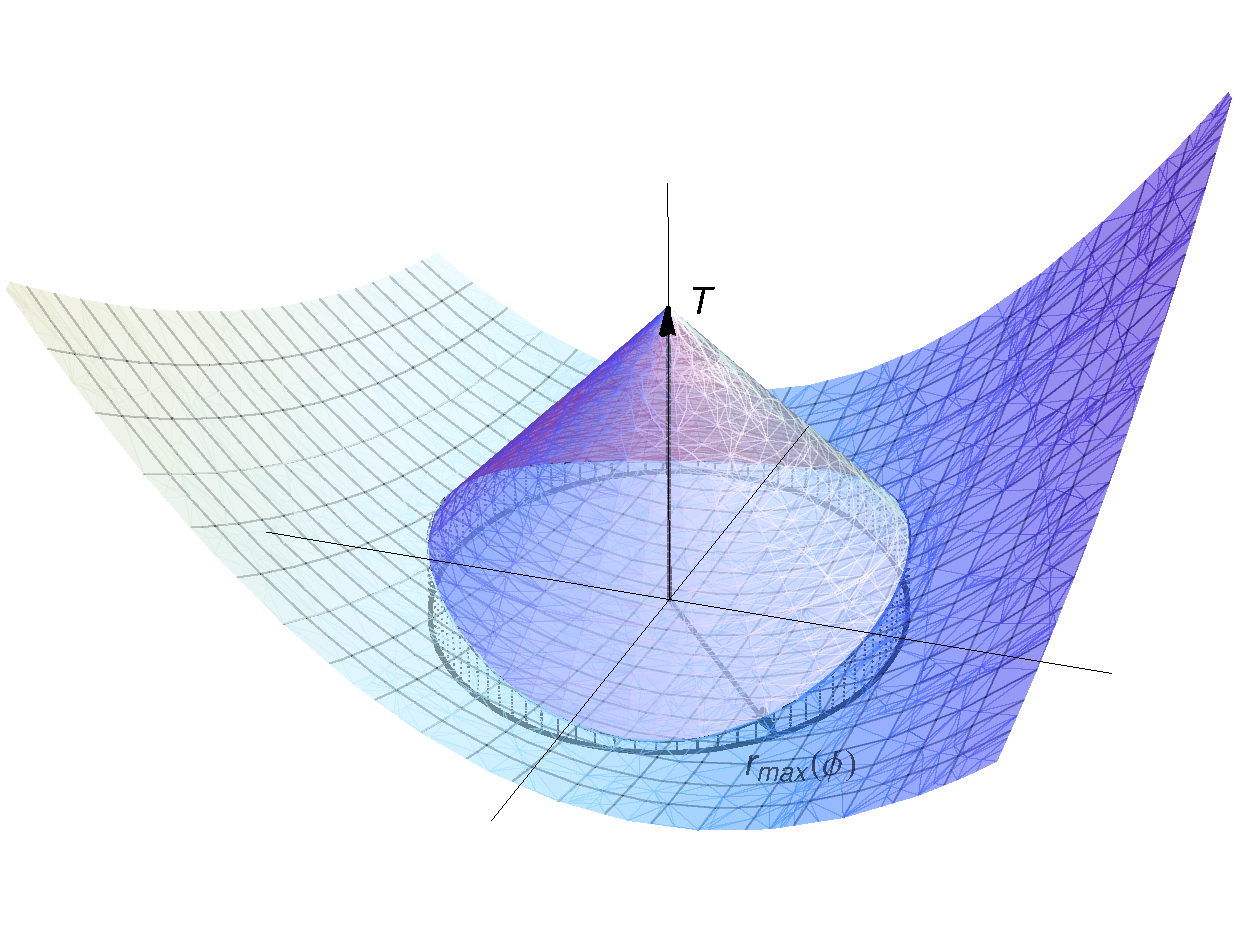
\includegraphics[scale=0.5]{coneplot}}
     \caption{The size of the region inside the top and bottom bounding surfaces is the volume we want to calculate.}
     \label{fig:cone_plot}
\end{figure}
\be\label{eq:VolumeNoK}
V_\blacktriangle(p)
=\frac{A_{d-2}}{d(d-1)}T^d\left(1-\frac{d}{2(d+1)}\Gamma^{0}_{\;ij}(p_0)A^{i}_{\;\ibar}A^{j}_{\;\jbar}\delta^{\ibar\jbar}T\right)
+O(T^{d+2})
\ee
where $A_{d-2}$ is the volume of the unit $(d-2)$-sphere and the $\delta^{\ibar\jbar}$ comes from the fact that cross terms ($\ibar\neq \jbar$) vanish under the angular integration. The defining relations for $A^{i}_{\;\ibar}$ can now be rearranged to give $A^{i}_{\;\ibar}A^{j}_{\;\jbar}\delta^{\ibar\jbar}=h^{ij}(p_0)$. Now in GNCs the extrinsic curvature on the surface is given by

\be\label{eq:K}
K
=g^{\mu\nu }\nabla_{\mu}n_{\nu}
=-\Gamma^{0}_{\;ij}h^{ij}=-\frac{1}{2}\frac{\dot{h}}{h}.
\ee
Substituting this into~\eqref{eq:VolumeNoK} with we obtain 
\begin{align}
V_\blacktriangle(T,\mathbf x)
&=\frac{A_{d-2}}{d(d-1)}T^d\left(1+\frac{d}{2(d+1)}K(0,\mathbf{x})T\right)
+O(T^{d+2}) \label{eq:TopVolumeWithK}\\
V_\blacktriangledown(-T,\mathbf x)
&=\frac{A_{d-2}}{d(d-1)}T^d\left(1-\frac{d}{2(d+1)}K(0,\mathbf{x})T\right)
+O(T^{d+2}), \label{eq:BottomVolumeWithK}
\end{align}
having dropped the subscript $p$. Given the volume expressions in GNCs we now proceed to evaluate the integrals for $\langle N_{min}^{(k)}\rangle $ and $\langle N_{max}^{(k)}\rangle$.

\subsection{The mean of $S^{(d)}_{GHY}[\mathcal C]$}

Using the previous equations for the volumes of the truncated cones we find that~\eqref{eq:nmax_and_eq:nmin} reduces to

\begin{gather}\label{eq:nmax_and_eq:nmin_volume_expanded}
\begin{aligned}
\langle N_{max}^{(k)}\rangle = \frac{\rho^{k+1}}{k!} & \int_{\Sigma}d^{d-1}x\int_{-\varepsilon}^{0}dt\:
h^{\frac{1}{2}}\left(1+
\frac{1}{2}\frac{\dot{h}}{h}t\right)
 \\
 & \times \Big( A(-t)^d \Big)^k 
 \Big( 1 - B(-t) \Big)^k
 e^{-\rho A(-t)^d \left[1-B(-t) \right]} + .\,.\,.
\\
\langle N_{min}^{(k)}\rangle = \frac{\rho^{k+1}}{k!} & \int_{\Sigma}d^{d-1}x\int_{0}^{\varepsilon}dt\:
h^{\frac{1}{2}}\left(1+
\frac{1}{2}\frac{\dot{h}}{h}t\right)
 \\
 & \times \Big( A\: t^d \Big)^k 
 \Big( 1 + B\: t \Big)^k
 e^{-\rho A\: t^d \left[1+B\: t \right]} + .\,.\,.
\end{aligned}
\end{gather}
where we have defined
\begin{gather}\label{A_and_B_defn}
\begin{aligned}
A & := \frac{A_{d-2}}{d(d-1)} \\
B & := \frac{A_{d-2}}{2(d-1)(d+1)}K(0,\mathbf{x})
\end{aligned}
\end{gather}
Once again the higher order terms that have been ignored in both equations will be shown to vanish in the limit. From~\eqref{eq:K} we can substitute $K$ in for $\frac{1}{2}\frac{\dot{h}}{h}t$. We swap the integration variable to $t\rightarrow -t$ in the first equation and expand the $O(t^{d+1})$ part of the exponentials to give

\begin{gather}\label{eq:nmax_and_eq:nmin_volume_expo_expanded}
\begin{aligned}
\langle N_{max}^{(k)}\rangle = \frac{\rho^{k+1}}{k!} & \int_{\Sigma}d^{d-1}x\int_{0}^{\varepsilon}dt\:
h^{\frac{1}{2}}\left(1+
K\: t\right)
 \\
 & \times \Big( A\: t^d \Big)^k 
 \Big( 1 - B\: t \Big)^k
 \Big( 1 + \rho A B\: t^{d+1} \Big)
 e^{-\rho A\: t^d} + .\,.\,.
\\
\langle N_{min}^{(k)}\rangle = \frac{\rho^{k+1}}{k!} & \int_{\Sigma}d^{d-1}x\int_{0}^{\varepsilon}dt\:
h^{\frac{1}{2}}\left(1-
Kt\right)
 \\
 & \times \Big( A\: t^d \Big)^k 
 \Big( 1 + B\: t \Big)^k
  \Big( 1 - \rho A B\: t^{d+1} \Big)
 e^{-\rho A\: t^d} + .\,.\,.
\end{aligned}
\end{gather}
The reason for expanding the exponentials is that the integrals will have to be put into the form of Gaussian integrals in order to evaluate them in the limit $\rho\rightarrow\infty$. The above expressions are almost the same apart from a few sign differences, so from now on we will just work with the expression for $\langle N_{min}^{(k)}\rangle$. By expanding the brackets, and retaining only necessary orders, the integral can be split into two parts of differing powers of $\rho$.

\begin{gather}\label{eq:n_min_different_rho_terms}
\begin{aligned}
\langle N_{min}^{(k)}\rangle & = \frac{\rho^{k+1}A^k}{k!}\int_{\Sigma}d^{d-1}x\: h^{\frac{1}{2}}\int_{0}^{\varepsilon}dt\:
\left\lbrace \left( t^{dk} + \left(kB-K \right)t^{dk+1}\right) + O\left(t^{dk+2}\right) \right\rbrace e^{-\rho A\: t^d}
 \\
 & - \frac{\rho^{k+2}A^{k+1}}{k!}\int_{\Sigma}d^{d-1}x\: h^{\frac{1}{2}}\int_{0}^{\varepsilon}dt\:
\left\lbrace Bt^{dk+d+1} + O\left(t^{dk+d+2}\right) \right\rbrace e^{-\rho A\: t^d}
\end{aligned}
\end{gather}
To find out how this diverges in the limit of $\rho \rightarrow\infty$, it suffices to find the divergence of the following general expression
\be\label{eq:general_t_n_integral}
\lim_{\rho\rightarrow\infty}\rho^{p}\int_{0}^{\varepsilon}dt\
t^{q}e^{-\rho At^{d}}
\ee
where $p,q \in \mathbb{R}$. We make the substitution $z=\rho At^{d}$ to put~\eqref{eq:general_t_n_integral} into the form of an incomplete gamma function.

\be\label{eq:incomplete_gamma_function}
\lim_{\rho\rightarrow\infty}\frac{A^{-\left(\frac{q+1}{d} \right)}}{d}\rho^{p-\left(\frac{q+1}{d} \right)}\int_{0}^{\rho A \varepsilon^d}dz\
z^{\left(\frac{q+1}{d} \right)-1}e^{-z}
\ee
The pre-factor has come from the substitution. In the limit we can retain the $\rho$ outside the integral while taking the integration limit to $\infty$. In doing this the integral becomes a gamma function.

\be\label{eq:gamma_function}
\lim_{\rho\rightarrow\infty}\frac{A^{-\left(\frac{q+1}{d} \right)}}{d}\rho^{p-\left(\frac{q+1}{d} \right)}\int_{0}^{\infty}dz\
z^{\left(\frac{q+1}{d} \right)-1}e^{-z}=\lim_{\rho\rightarrow\infty}
\frac{A^{-\left(\frac{q+1}{d} \right)}}{d}\rho^{p-\left(\frac{q+1}{d} \right)}\Gamma\left( \frac{q+1}{d} \right)
\ee
We can use this procedure to take the limit of~\eqref{eq:n_min_different_rho_terms} and formulate the answer in terms of gamma functions. The limits of both $\langle N_{min}^{(k)}\rangle$ and $\langle N_{min}^{(k)}\rangle$ are then given by

\begin{gather}\label{eq:nmax_nmin_final}
\begin{aligned}
\lim_{\rho\rightarrow\infty}\langle N_{max}^{(k)}\rangle = \lim_{\rho\rightarrow\infty} & \left\lbrace \rho^{1-\frac{1}{d}} \left(b_d\right)^{-1} \frac{\Gamma\left(\frac{1}{d}+k\right)}{k!}
\int_{\Sigma}d^{d-1}x\: \sqrt{h} \right.
 \\
 &  \left. +\rho^{1-\frac{2}{d}} \left(c_d\right)^{-1} \frac{\Gamma\left(\frac{2}{d}+k\right)}{k!}
\int_{\Sigma}d^{d-1}x\: \sqrt{h}K + O\left(\rho^{1-\frac{3}{d}} \right) \right\rbrace
\\
\lim_{\rho\rightarrow\infty}\langle N_{min}^{(k)}\rangle = \lim_{\rho\rightarrow\infty} & \left\lbrace \rho^{1-\frac{1}{d}} \left(b_d\right)^{-1} \frac{\Gamma\left(\frac{1}{d}+k\right)}{k!}
\int_{\Sigma}d^{d-1}x\: \sqrt{h} \right.
 \\
 &  \left. -\rho^{1-\frac{2}{d}} \left(c_d\right)^{-1} \frac{\Gamma\left(\frac{2}{d}+k\right)}{k!}
\int_{\Sigma}d^{d-1}x\: \sqrt{h}K + O\left(\rho^{1-\frac{3}{d}} \right) \right\rbrace
\\
\end{aligned}
\end{gather}

These object diverge as $\rho^{1-\frac{1}{d}}$ in the limit. The factor of $\rho$ that must be included in the formula for the surface volume is exactly the inverse of this ($\rho^{\frac{1}{d}-1}$), as can be seen from~\eqref{eq:surface_volume} if one substitutes in $l=\rho^{-\frac{1}{d}}$. If we include this factor above and then take the limit we see that the only remaining terms are proportional to the surface volume. The other terms all have negative powers of $\rho$ and therefore vanish as $\rho\rightarrow\infty$. From this it follows that the mean of any linear combination of terms like $\rho^{\frac{1}{d}-1}\langle N_{max}^{(k)}\rangle$ or $\rho^{\frac{1}{d}-1}\langle N_{min}^{(k)}\rangle$ will give something proportional to the surface volume, so long as the terms containing the surface volume don't exactly cancel. To simplify the coefficients in this linear sum we take out a factor of $\frac{k!}{\Gamma\left(\frac{1}{d}+k\right)}$. The last step in arriving at~\eqref{general_area_sum} is to enforce the condition that the coefficients sum to unity, in order for the linear sum to equal the surface volume and not just be proportional. This concludes the proof of the surface volume conjecture. 

If we multiply~\eqref{eq:nmax_nmin_final} by the appropriate factor of $\rho$ from the boundary term ($\rho^{\frac{2}{d}-1}$) we find that the above equation still diverges as $\rho^{\frac{1}{d}}$ in the limit. This divergence comes from the surface volume term, while the term proportional to the GHY boundary term is finite. In order to recover the boundary term we must take a linear combination of these objects such that the term proportional to the surface are vanishes, while the term proportional to the boundary term does not. This is where the condition~\eqref{coefficient_relation} comes in. This condition for the coefficients is only so simple because we have taken out a factor of $\frac{k!}{\Gamma\left(\frac{1}{d}+k\right)}$ from each coefficient. The remaining sum is proportional to the boundary term, and in order to get it exactly we simply have to divide out by the proportionality constant. At this point one arrives at~\eqref{general_boundary_sum} and the proof is concluded.

\section{Fluctuations}
So far we have only talked about the mean of the causal set boundary action. Let us now turn to its fluctuations (the standard deviation) $\sigma[S^{(d)}_{GHY}(\mathcal C)]=\text{Var}[S^{(d)}_{GHY}(\mathcal C)]^\frac12$.\footnote{Whenever we say fluctuations we refer to the standard deviation of the random variable, not to its variance.} We can make a heuristic argument to estimate the dependence of fluctuations on $\rho=l^{-d}$. In any spacetime region of fixed volume $V$ the number of causal set elements $N$ experiences Poisson fluctuations of order $\sqrt N$. We will use the first case of~\eqref{GH_boundary_to_causet} as it is the simplest case in which to make this argument for the fluctuations. Since $N_{max}^{(0)}$ and $N_{min}^{(0)}$ are quantities associated with a codimension-1 surface (they count elements ``near" $\Sigma$), we may expect them to scale like $N^\frac{d-1}{d}$ --- which agrees with the leading order behaviour of~\eqref{eq:nmax_nmin_final} --- and thus to inherit fluctuations of order $N^\frac{d-1}{2d}$. 
%{This comes from the following observation. In a volume corresponding to a thickening of the hypersurface $\Sigma$ by one unit of the discreteness scale $l$ (e.g. by Lie dragging the surface along its normal by an amount $l$),.... }
The action $S^{(d)}_{GHY}$, being proportional to $\rho^\frac{2-d}{d}$ times the difference of two independent\footnote{The independence is as a feature of the Poisson process in $M$: the number of elements $N(R)$ in any subregion $R\subset M$ is a Poisson variable itself, and for any two disjoint regions $R_1$, $R_2$ the numbers $N(R_1)$ and $N(R_2)$ are independent random variables.} random variables with standard deviation $N^\frac{d-1}{2d} = (\rho V)^\frac{d-1}{2d}$ should see fluctuations of order $\rho^\frac{2-d}{d}\rho^\frac{d-1}{2d}=\rho^\frac{3-d}{2d}$. This suggests that for $d=2$ these fluctuations should grow like $\rho^{\frac{1}{4}}$ as $\rho\rightarrow\infty$, for $d=3$ they should be constant, and for $d>3$ they should be damped.

In order to test this heuristic argument one may like to write down the integral expression for $\text{Var}[S^{(d)}_{GHY}(\mathcal C)]^\frac12$ but it is complicated enough even in finite regions of flat space for which it is not very illuminating to reproduce here. It also seems far less tractable than the expression for the mean because it involves terms of the type $\int d^dx\int d^dy \exp\left[-\rho V(J^+(x)\cap J^+(y))\right]$ for which the above methods of cutting off the time-integration range and Taylor expanding will not follow through. Instead we will show the results of computer simulations that support results of the heuristic argument. 

\begin{figure}[t!]
  \centering
    {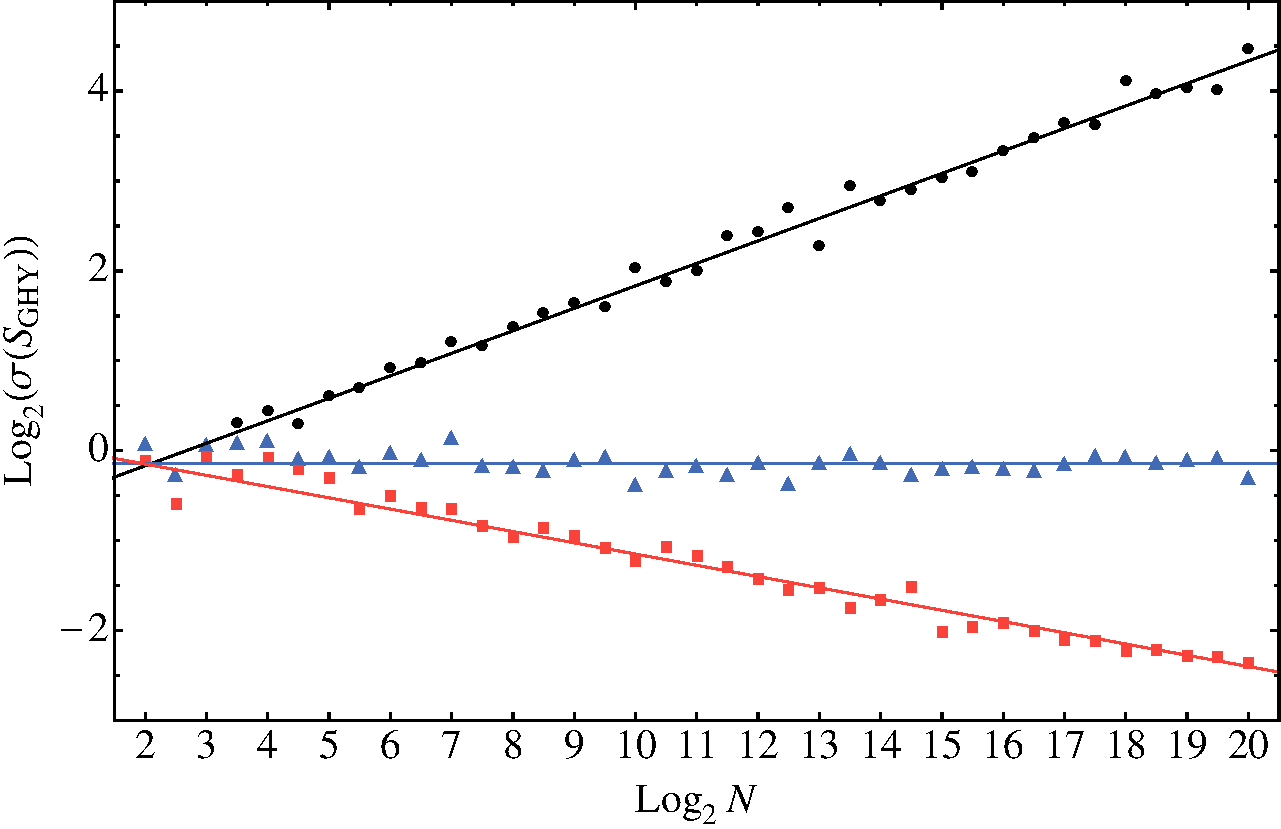
\includegraphics[scale=0.6]{GHY-fluctuation_plots}}
     \caption{A $\log-\log$ plot (base $2$) of the fluctuations in $S^{(d)}_{GHY}$ for a flat ($K=0$) surface in $d=2,3$ and $4$-dimensional Minkowski space. Each data point represents the sample standard deviation in $S^{(d)}_{GHY}$ on a sample of $R=100$ runs. Black dots, blue triangles and red squares correspond to the simulation results in $d=2,3$ and $4$ dimensions, respectively. The corresponding black, blue and red lines have gradients $\frac12$, $0$ and $-\frac18$ and best-fit intercepts of order $1$.}
     \label{fig:fluctuations}
\end{figure}

 
The simulations were carried out as follows. Denote the discreteness scale by $l$. Take a $d$-cube $[0,L]^d$ in $d$-dimensional Minkowski space with metric $ds^2=-dt^2+d{\mathbf x}^2$ and define the hypersurface $\Sigma: t=L/2$, which partitions the cube into two equal halves. Sprinkle at density $\rho=l^{-d}$ into the cube, which in any given run will place $N$ points inside the cube where $N$ is a Poisson random number with mean $\langle N\rangle = \rho V=  (L/l)^d$. Evaluate $S^{(d)}_{GHY}=\rho^\frac{2-d}{d}c_d\left(2\Gamma\left(\frac{2}{d}\right)\right)^{-1}(N_{max} - N_{min})$ for $\Sigma$ by counting the minimal/maximal elements in the upper/lower half of the cube, and repeat for $R$ runs. The expected value for the mean is zero in all cases, since the extrinsic curvature of the surface is zero. 

In Figure~\ref{fig:fluctuations} we display the simulation results for $d=2,3,4$ spacetime dimensions, with $N=\rho$ ranging up to $2^{20}\approx 1$ million, having set $V=L^d=1$. Each data point represents the fluctuations (the standard deviation) in a sample of $R=100$ runs. The solid lines have been obtained by fitting an arbitrary constant multiplier in the scaling law predicted by the argument above, $\gamma(d)\times N^\frac{3-d}{2d}$, to the data sets. The best fit values are all of order $1$: $\gamma(2)=0.63$, $\gamma(3)=0.91$, and $\gamma(4)=1.07$.
There is clearly a good fit between the data and the scaling predicted by the heuristic argument. Although not visible on the plot, the data points were all consistent with zero mean as well.

We have performed analogous simulations for the second formula in~\eqref{GH_boundary_to_causet}, involving $N^{(1)}_{max}$ and $N^{(0)}_{max}$. In this case, heuristic arguments of the type given above are hampered by the fact that the two random variables whose difference is taken are not independent. However, the results for the scaling of the fluctuations turn out to be identical to those obtained in the first case. 

\section{A Candidate Boundary Term for an Alexandrov Interval}


Until now our approach has been to reconstruct the  continuum GHY term  from the information in a causal set. 
The candidate described in the previous sections for a spatial boundary has a natural expression in a causal set  in  terms of its maximal and minimal elements which are the  analogs of a  space-like boundary.  A suitable analog  of  a time-like boundary  term has been harder to  construct; there is no simple causal set  characterisation of a time-like boundary. Indeed, it seems difficult to characterise a causal set in a  spacetime region which is bounded by time-like surfaces. On the other hand, since past and future sets are natural in a causal set, such regions do find a natural characterisation in a causal set. An important example of such a region is the  Alexandrov interval which is used extensively  in calculations of causal set kinematics.  In the continuum such a region  is bounded by null hypersurfaces and their spatial joints.  

Conversely in the continuum,   while the GHY term  is well defined for both a space-like and time-like boundary,  including their co-dimension 2 joints \cite{harris},  it is an open question what the contribution from a null  boundary  is \cite{ghh}. Apart from some sketchy suggestions in the literature \cite{neiman} there is no rigourous construction of such a term; indeed the standard variational route for finding the boundary contribution to the action appears to fail for null boundaries. 

Given the lack of a  null GHY term, we can ask if causal set theory  might  in fact guide us in the right direction.   Our starting point is the $d$-dimensional  Benincasa-Dowker Action \cite{bd,gd} which is constructed from the mean number  $N_i^{(d)}$ \footnote{ $N_i^{(d)}$ is dimension  and geometry dependent, but for our purpose it suffices to retain the dimension label. } of $i+1$-element inclusive intervals in the causal set 
\begin{equation} 
8 \pi G {S_{BD}^d} = -\alpha_d \rho^{\frac{2-d}{d}}\biggl( N+ \frac{\beta_d}{ \alpha_d} \sum_{i=1}^{n_d-1}  C^{(d)}_{i} N _i^{(d)} \biggr) 
\label{bd} 
\end{equation}  
where   
\begin{equation} 
 \alpha_d= \left \{ %
\begin{array} {ccc}
-\frac{1}{\Gamma(\frac{2+d}{d})}c_d ^{2/d}  & \quad &  \mathrm{d} \, \, \mathrm{odd} \\
-2 \frac{1}{\Gamma(\frac{2+d}{d})}c_d ^{2/d} & \quad &  \mathrm{d \, \,  even} \\
\end{array} \right  
\quad \beta_d = \left \{ 
\begin{array} {ccc}
\frac{d+1}{2^{d-1}\Gamma(2/d +1)} c_d^{2/d}  & \quad &  \mathrm{d \, \, odd}\\ 
\frac{\Gamma(d/2+2)\Gamma(d/2+1)}{\Gamma(2/d)\Gamma(d)}c_d^{2/d}  & \quad & \mathrm{d \, \,  even}\\ 
\end{array} \right 
\end{equation} 
\begin{equation} 
n_d = \left \{ %
\begin{array} {ccc}
\frac{d-1}{2} + 2 & \quad &  \mathrm{d \, \, odd}\\ 
\frac{d}{2} + 2 & \quad & \mathrm{d \, \,  even}\\ 
\end{array} \right 
\end{equation} 
with $2^{-d/2} c_d$ is the volume of a unit Alexandrov interval $I(x,y)$, i.e., one for which the proper time $\tau(x,y)=1$. 
%%{ {\bf \color{red} this is not correct! $c_d= vol(S_{d-2}) \frac{ 2^{\frac{2-d}{2}}}{d(d-1)}$ and $vol(S_{d-2})$ the volume of the homogeneous $d-2$ sphere}}.  
The coefficients  of $N_i^{(d)}$ in the sum are are 
\begin{equation}
\label{cid}
 C_i^d= \left \{ %
\begin{array} {ccc}
\sum_{k=0}^{i-1} (-1)^k\binom{i-1}{k} \frac{\Gamma(d/2(k+1)+3/2)}{\Gamma(d/2+3/2) \Gamma(1+dk/2)} & \quad &  \mathrm{d \, \, odd}\\ 
\sum_{k=0}^{i-1} (-1)^k\binom{i-1}{k} \frac{\Gamma(d/2(k+1)+2)}{\Gamma(d/2+2) \Gamma(1+dk/2)} & \quad & \mathrm{d \, \,  even}\\ 
\end{array} \right 
\end{equation} 
These coefficients can be expressed more compactly as hypergeometric functions 
\begin{equation}
C_i^d={}_{q+1}F_{q}(\{ a_1, \ldots a_q, i-1\}, \{b_1, \ldots b_q \} |1)
\label{chyp} 
\end{equation} 
with $q=d/2+1/2, a_i=\frac{d+2i}{d}, b_i=2i/d$ for $d$ odd and $q=d/2, a_i=\frac{d+2i+2}{d}, b_i=2i/d$  for $d$ even.  


If $S_{BD}^d$ were precisely the discrete analog of the Einstein Hilbert action {\it without} any boundary contributions, then in Minkowski spacetime  $S_{BD}^d$ should  vanish. However, as shown explicitly in \cite{bbdtwo} this is not the case for Alexandrov intervals in 2$d$  Minkowski spacetime. Indeed, there is a residual contribution that goes to a constant in the continuum limit $N\rightarrow \infty$.  When the action is evaluated in rectangular regions in the same spacetime or for Alexandrov intervals in  the flat trousers spacetime, this is no longer the case. Thus, it seems plausible that the 2$d$ BD action contains some boundary information. Moreover, in the large $N$ limit  the action goes to the same  non-vanishing constant irrespective of the interval size. While this might suggest a non-geometric or topological origin, we will now show that it is a part of a universal  behaviour for higher $d$ and in fact  has a geometrical origin. 

Consider an Alexandrov interval $I(p,q)=I^+(p) \cap I^-(q)$ for two events $p,q$ in a causal spacetime.   While the  boundary of $I(p,q)$ may be quite complicated in general, some of these components must necessarily be null.  In Minkowski spacetime, for example,  the boundary of $I(p,q)$ consists of the two events $p$ and $q$, the subsets $B^\pm$ of the  two null hypersurfaces $\partial J^+(p)$ and $\partial J^-(q)$, and their intersection or ``joint''  $S_{d-2}=\partial J^+(p) \cap \partial J^-(q)$ which is a codimension 2 sphere.  Evaluating the BD action for an Alexandrov interval in flat spacetime should therefore give us terms that are only dependent on the boundary components.  In flat spacetime the $S_{d-2}$ joint  has radius $\tau(p,q)/2$, and thus increases with the size of the Alexandrov interval ${\mathrm{vol}}(I(p,q)) = N/\rho$, where $N$ is the mean of the number of causal set elements sprinkled into $I(p,q)$ . In what follows we take the continuum limit $\rho, N \rightarrow \infty$ while keeping ${\mathrm{vol}}(I(p,q))$ fixed. \mnote{\color{red} SS: It would be nice to have a fancy picture of an Alex. interval here..}  
%% If $p$ or $q$ were to be taken to time-like past or future infinity, this volume would go to infinity as expected.

In \cite{glasersurya} a closed form expression was obtained for the mean value of the number of $i+1$ element inclusive intervals  $N_i^d$ contained in an  Alexandrov interval in $d$ dimensional Minkowski  spacetime 
\begin{equation} 
N_i^d= \frac{\Gamma(d)^2}{\Gamma(i)} \sum_{k=0}^\infty \frac{(-1)^k}{\Gamma(k+1)} \frac{N^{k+i+2}}{(k+i+2)(k+i+1)} \frac{\Gamma(\frac{d(k+i)}{2}+1) \Gamma(\frac{d(k+i+1)}{2}+1)}{\Gamma(\frac{d(k+i)}{2} +d) \Gamma(\frac{d(k+i+1)}{2}+d)}, 
\end{equation}
where $i \geq 1$.   In taking the $N \rightarrow \infty$ limit, it   is convenient to consider the ratio
\begin{equation} 
\frac{ 8 \pi G S^d(C)}{vol(S^{d-2})} = \frac{b}{d(d-1) \Gamma(1+2/d) N^{\frac{d-2}{d}}} \left( N + \frac{\beta_d}{\alpha_d} \sum_{i=1}^{n_d} C_i^d N_i^d \right)  
\label{ratio} 
\end{equation} 
where $b=1$ for $d$ odd and $b=2$ for $d$ even. 
We use Mathematica to evaluate the $N \rightarrow \infty$  limit of this expression for $d=2, \ldots 9$. We aid the calculation by expanding the sum  $\sum_{i=1}^{n_d} C_i^d N_i^{(d)} = \sum_{j=1}^\infty A_j^d N^{j+1}$ as a  power series in  $N$. After a rearrangement and redefinition of indices we find that 
\begin{equation}
 A_j^d = \Gamma(d)^2\biggl( \sum_{i=1}^{D+2} (-1)^i \binom{j-1}{i-1}  C_i^d  \biggr) \frac{(-1)^j}{(j+1)!}\frac{\Gamma(\frac{d}{2}(j-1)+1)\Gamma(\frac{d}{2}j+1)}{\Gamma(\frac{d}{2}(j-1)+d) \Gamma(\frac{d}{2}j+d)}, 
\end{equation} 
where $d=2D$ for $d$ even and $d=2D+1$ for $d$ odd.   
% Using the abbreviated form $C_i^d=\sum_{l=0}^{i-1} \binom{i-1}{l}A(d,l)$ where $A(d,l)$ is defined using \ref{cid} 
% we find that 
% \begin{equation}
% \sum_{i=1}^{D+2} (-1)^i \binom{j-1}{i-1}  C_i^d = (-1)^{j-1} A(d,j-1),  
% \end{equation}      
% where we have used the binomial identities  BLAH. Thus 
% \begin{equation}
%  \sum_{i=1}^{n_d} C_i^d N_i^{(d)}= ((d-1)!)^2 \sum_{j=1}^\infty(-1)^j B(d,j) \frac{\Gamma(\frac{d}{2}j+1)}{\Gamma(j+2)\Gamma(\frac{d}{2}(j-1)+d)\Gamma(\frac{d}{2}j+d)}N^{j+1}
% \label{thesum} 
% \end{equation} 
% where 
% \begin{equation} 
% B(d,j) = \left \{ 
% \begin{array}{ccc} 
% \frac{\Gamma(\frac{d}{2}j+3/2)}{\Gamma(\frac{d}{2}+3/2)}  &\quad & d \, \, odd, \\  \frac{\Gamma(\frac{d}{2}j+2)}{\Gamma(\frac{d}{2}+2)}  &\quad & d \, \, even.  \\ 
% \end{array} 
% \right
% \end{equation} 
An explicit  calculation of $8\pi S_{BD}^d$ in $I(p,q)$ for $d=2, \ldots 9$  gives 
\begin{equation} 
\lim_{N \rightarrow \infty} \frac{ 8 \pi G S_{BD}^d(C)}{vol(S^{d-2})} = 1,  
\label{result} 
\end{equation} 

\mnote{\color{red} SS: There are further simplifications I have that may help mathematica for $n>9$. It is still not clear}  Since $N_i^d$ can also be expressed as a hypergeometric function, using  (\ref{chyp}) it   is seems possible to evaluate (\ref{ratio}) using identities involving sums of products of such functions to get a closed form expression for arbitrary $d$.  In \cite{glasersurya} the asymptotic form of $N_i^d$ was explicitly calculated, and for $d>2$, the leading order was shown to  $~ N^{2-\frac{2}{d}}$ which dominates $N$ dependence for $d>2$. To be consistent with  (\ref{result}) this would mean that the leading order contributions from the $N_i^d$ cancel in the action. This is indeed explicitly seen to be the case, again for $d=3, \ldots 9$. Similarly, for $d=2$, where the leading order contribution is $~ N \log N$.  Indeed, in all cases the next to leading order terms given in \cite{glasersurya} also do not have the requisite $~N^{\frac{d-2}{d}}$ dependence required by (\ref{result}); in this case, the explicit coefficients are not available to   check that they give a vanishing contribution to (\ref{result}).  This suggests that  we cannot rely   on the the asymptotic form of the individual terms  in the sum  for an analytic proof for general $d$, which could therefore be quite non-trivial. 

The result we have obtained is for flat spacetime. One may speculate that the presence of curvature will not modify the essential result, i.e., that the only boundary contribution is from the volume of the spatial $d-2$ sphere at the joint, at least in the case when the boundary consists of the same type of components.   What will change of course is the fact that the principal radii of the $d-2$ sphere could be different at  every point, hence complicating the relationship between the volume of the interval and the volume of this sphere. In  \cite{Khetrapal_Sumati:Causal_Diamond_Volume} it was shown that in an RNC, to first order in curvature, 
the intrinsic boundary geometry of the Alexandrov interval is still flat which would simplify this relationship. Using an RNC version of the calculation  one could thus make an explicit calculation possible. 

The fact that the BD action does not vanish in flat spacetime suggests  that this action  does not only code information about the bulk Einstein Hilbert action but also contains  extra boundary information in general.  One might then be tempted to speculate that it contains {\it all} the relevant boundary information suggesting that the null boundary contribution for an Alexandrov interval in any spacetime always vanishes. Moreover, in the specific case that there is only a single spatial component coming from the joint, that the only boundary contribution is the volume of this $d-2$ sphere.  comes from this  that (\ref{result}) gives the GHY contribution for an Alexandrov interval.

\newpage

\bibliographystyle{jhep}

\bibliography{references}

\end{document}


%%
JHEPPUB:

\title{Gibbons-Hawking-York Boundary Term in Causal Sets}
 \author[a]{M. Buck}
 \author[a,b]{\!, F. Dowker}
 \author[a]{and I. Jubb\,}
\affiliation[a]{Theoretical Physics Group, Blackett Laboratory, Imperial College, London, SW7 2AZ, U.K.}
\affiliation[b]{Institute for Quantum Computing, University of Waterloggedo, ON, N2L 2Y5, Canada}

\abstract{ 
We show some stuff.
}

\begin{document}

\maketitle

\pagebreak

\noindent NOTES:\\
1. define s as the RV, not as its mean

\section{Introduction}




%%IOPART

\begin{document}

\title{Gibbons-Hawking-York Boundary Term in Causal Sets}

\author{Michel Buck Fay Dowker, Ian Jubb}
\address{Blackett Laboratory, Imperial College, London, SW7 2AZ, U.K.}

\begin{abstract}

We show some stuff.

\end{abstract}
%\pacs{03.67.-a, 03.65.Ta, 03.70.+k}

\maketitle
\section{Introduction}
%%